\documentclass[11pt,a4paper]{ivoa}
\input tthdefs

\SVN$Rev$
\SVN$Date$
\SVN$URL$


\iftth
\newenvironment{args}%
{\begin{html}<ul>\end{html}\def\arg##1(##2){\begin{html}<li><i>\end{html}%
  ##1 \begin{html}</i>(<code>\end{html}##2\begin{html}) </code>\end{html}}}%
{\begin{html}</ul>\end{html}}
\else
\newenvironment{args}%
% this is *only* for use within a description environment
  {\hfil % let definition label stand on a line of its own.
    \def\arg##1(##2){\item {\textit{##1} (\texttt{##2})}}
    \begin{list}{$\bullet$}{\topsep=0pt\partopsep=0pt\parsep=0pt}
    }%
  {\end{list}}
\fi

\title{Catalogue of ADQL User Defined Functions}

% see ivoatexDoc for what group names to use here
\ivoagroup{DAL}

\author{Jon Juaristi Campillo}
\author[https://wiki.ivoa.net/twiki/bin/view/IVOA/MarkusDemleitner]{Markus Demleitner}


\editor{Jon Juaristi Campillo}

% \previousversion[????URL????]{????Funny Label????}
\previousversion{This is the first public release}
       

\begin{document}
\begin{abstract}
The endorsed content of this note documents the consensus on ADQL user
defined functions (UDFs) with an \verb|ivo_| prefix, either by
referencing recommendations that defined the function, or by defining
functions in place.  A non-normative appendix lists UDFs declared by
registered TAP services.
\end{abstract}


\section*{Conformance-related definitions}

The words ``MUST'', ``SHALL'', ``SHOULD'', ``MAY'', ``RECOMMENDED'', and
``OPTIONAL'' (in upper or lower case) used in this document are to be
interpreted as described in IETF standard RFC2119 \citep{std:RFC2119}.

The \emph{Virtual Observatory (VO)} is a
general term for a collection of federated resources that can be used
to conduct astronomical research, education, and outreach.
The \href{http://www.ivoa.net}{International
Virtual Observatory Alliance (IVOA)} is a global
collaboration of separately funded projects to develop standards and
infrastructure that enable VO applications.


\section{Introduction}

The Astronomical Data Query Language ADQL \citep{2008ivoa.spec.1030O}
has the notion of user defined fucntions (UDF).  These provide a
light-weight extension mechanism for operators of TAP services.  
For instance, \citet{2016arXiv161109190T} shows how they enable the
construction of HEALPix maps although ADQL~2.0 itself entirely lacks
facilities to deal with them.

In order to provide a reliable core set of such functions that, if
present, have a constant meaning across multiple services, ADQL 2.1
(still under review at the time of writing) will stipulate that user
defined functions with names starting with \verb|ivo_| are to be used
and defined interoperably, i.e., there should be an IVOA-wide consensus
on their names and semantics. 

This note documents this consensus where it has been reached within
other standards.  Where UDFs are not naturally associated to a
particular standard, they can be proposed by editing this document and
starting the Endorsed Note process \citep{2017ivoa.spec.0517G} on the
changes.  In effect, this endorsed note is the management tool for
the \verb|ivo_| ``namespace'' in ADQL user defined functions.

Note that no function given here is required to be present in a generic
TAP service (though other standards may pose such requirements;
\verb|ivo_hashlist_has|, for instance, is, or will be, required by both
RegTAP and EPN-TAP).  However, if a service implements any UDF with a
name starting with \verb|ivo_|, its semantics must be as specified here.

Informationally, in each revision of this document, we also run an
all-VO survey of user defined functions in registered TAP services.  The
result of this survey is available as an appendix (which, by
construction, is non-normative).

%\subsection{Role within the VO Architecture}

%\begin{figure}
%\centering

%% As of ivoatex 1.2, the architecture diagram is generated by ivoatex in
% SVG; copy ivoatex/archdiag-full.xml to archdiag.xml and throw out
% all lines not relevant to your standard.
% Notes don't generally need this.  If you don't copy archdiag.xml,
% you must remove archdiag.svg from FIGURES in the Makefile.

%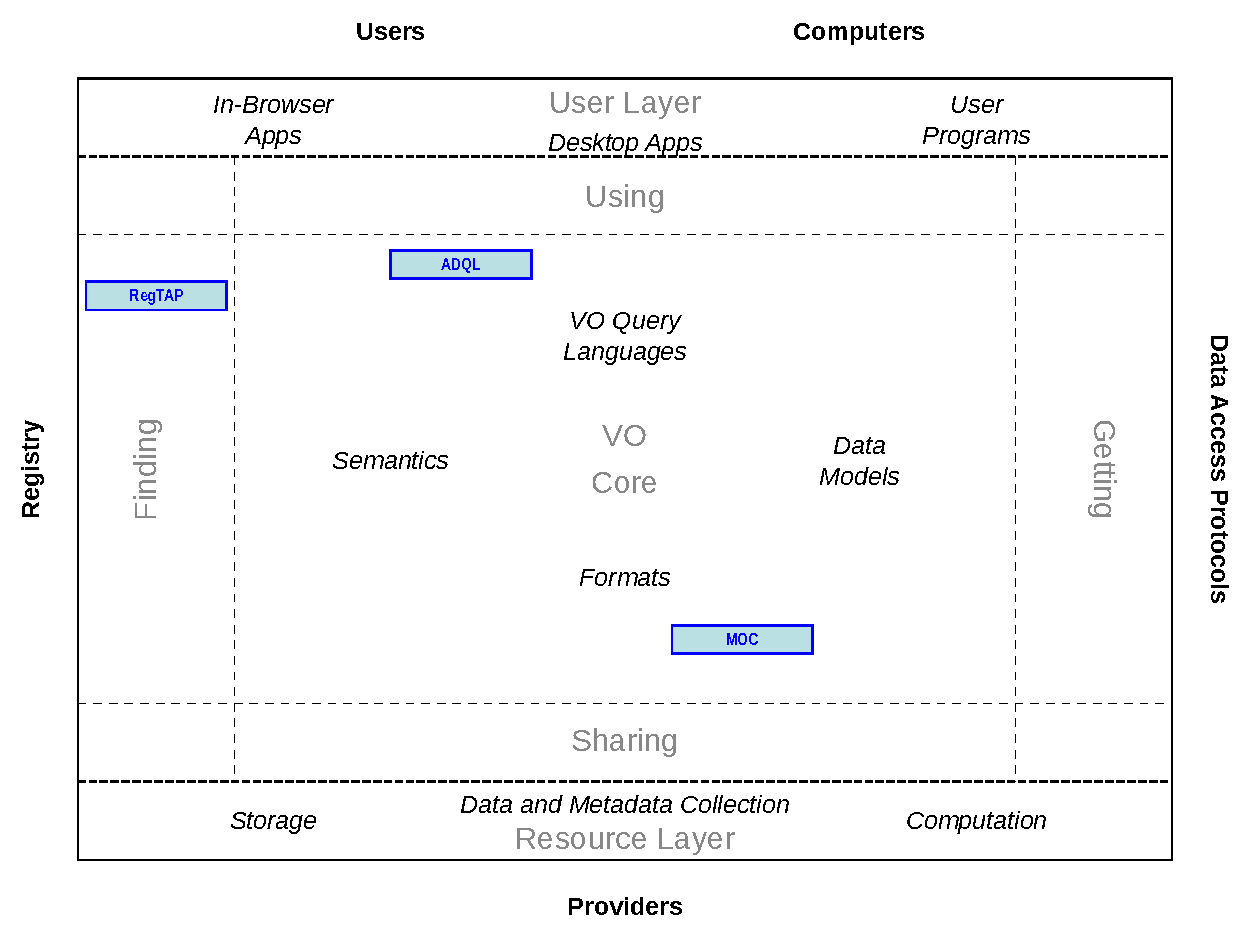
\includegraphics[width=0.9\textwidth]{role_diagram.pdf}
%\caption{Architecture diagram for this document}
%\label{fig:archdiag}
%\end{figure}

%Fig.~\ref{fig:archdiag} shows the role this document plays within the
%IVOA architecture \citep{note:VOARCH}.


\section{List of IVOA user defined functions}

The functions are defined through a brief human-readable description of
what the function does, followed by a closer discussion of the
parameters, the return value, and the source of UDF.

In the parameter definitions, we do not distinguish between different
lengths of floating point arguments.  Where we write \texttt{REAL}, the
expectation is that the functions accept floating point values of any
length.


\subsection{HEALPix-related}

In this section, order and npix are used as in the MOC recommendation
\citep{2014ivoa.spec.0602F}.

\subsubsection{ivo\_healpix\_index(hpxOrder, long, lat)}

Returns the index (npix) of the Healpix cell containing the spherical
point given by longitude \texttt{long} (typically, RA) and latitude
\texttt{lat} (typically, declination) at order \texttt{hpxOrder} in
NESTED numbering.

\begin{description}
\item[Parameters]
\begin{args}
	\arg hpxOrder (INTEGER) -- the HEALPix order to use.
	\arg ra (REAL) -- longitude of the spherical point to compute the
	index for, in degrees.
	\arg dec (REAL) -- latitude of the spherical point to compute the
	index for, in degrees.
\end{args}

\item[Return type] \texttt{BIGINT}

\item[Source] This document.
\end{description}

\subsubsection{ivo\_healpix\_index(spoint)}

Returns the index (npix) of the HEALPix cell containing the spherical
point given by \texttt{spoint} at order \texttt{hpxOrder} in NESTED
numbering.

\begin{description}
\item[Parameters]
\begin{args}
	\arg hpxOrder (INTEGER) -- the HEALPix order to use.
	\arg spoint (POINT) -- the position to compute the index for.
\end{args}

\item[Return type] \texttt{BIGINT}

\item[Source] This document.
\end{description}

\subsubsection{ivo\_healpix\_center(hpxOrder, hpxIndex)}

Returns a POINT corresponding to the center of the HEALPix cell
with index (npix) \texttt{hpxIndex} at order \texttt{hpxOrder}.

\begin{description}
\item[Parameters]
\begin{args}
	\arg hpxOrder (INTEGER) -- the HEALPix order to use.
	\arg hpxIndex (INTEGER) -- the index for which to return the center
	position.
\end{args}

\item[Return type] \texttt{POINT}

\item[Source] This document.
\end{description}

\subsubsection{ivo\_apply\_pm(ra, dec, pmra, pmdec, epochDist)}

Returns a POINT for the position an object at \texttt{ra},
\texttt{dec} will be at after \texttt{epochDist} Julian years if its proper
motion is \texttt{prma}, \texttt{pmdec}.  Positions must be in degrees,
proper motions are expected in degrees/year. The proper motions must be
given in the tangential plane (,,contain $cos(\delta)$'').

Note that this is an operation of spherical geometry, i.e., the function
would work as well with non-equatorial coordinates \emph{and} proper
motions.  However, you cannot, of course, mix galactic coordinates with
equatorial proper motions.


\begin{description}
\item[Parameters]

\begin{args}
	\arg ra (REAL) -- longitude of the spherical position, in degrees.
	\arg dec (REAL) -- latitude of the spherical position, in degrees.
	\arg pmra (REAL) -- proper motion in longitude in the
	tangential plane (i.e., the simple derivative has been divided by
	cos(dec)), in degrees per Julian year.
	\arg pmdec (REAL) -- proper motion in latitude, in degrees per Julian
	year.
	\arg epochDist (REAL) -- propagate the object this many Julian years.
\end{args}

\item[Return type] \texttt{POINT}

\item[Source] This document.
\end{description}


\subsection{Text related}

\subsubsection{ivo\_string\_agg(expression, delimiter)}

An aggregate function returning all values of \texttt{expression} 
concatenated with delimiter.

\begin{description}
\item[Parameters]

\begin{args}
	\arg expression (TEXT) -- a SQL expression giving the strings to
	concatenate.  The expression may be NULL, in which case the row does
	not leave a trace in the result string.
	\arg delimiter (TEXT) -- a string used to concatenate the values of
	\texttt{expression} in each group.
\end{args}

\item[Return type] \texttt{TEXT}

\item[Source] RegTAP \citep{2014ivoa.spec.1208D}
\end{description}

\subsubsection{ivo\_nocasematch(value, pattern)}

Evaluates \verb value ILIKE pattern, i.e.,
pattern is defined as for the SQL LIKE operator, but the match is
performed case-insensitively.  Returns
1 if the pattern matches, 0 otherwise.

In ADQL 2.1 and later, use the ILIKE operator instead.

\begin{description}
\item[Parameters]

\begin{args}
	\arg value (TEXT) -- a string-valued SQL expression.
	\arg pattern (TEXT) -- a SQL pattern for LIKE evaluation (i.e.,
	underscore is any character, percent zero or more arbitrary
	characters).
\end{args}

\item[Return type] \texttt{INTEGER}

\item[Source] RegTAP \citep{2014ivoa.spec.1208D}
\end{description}

\subsubsection{ivo\_hasword(haystack, needle)}

Returns 1 if the string \texttt{needle} is contained (in some sense) in
the string \texttt{haystack}, 0 otherwise.  This is intended to support
somewhat ``Google-like'', soft string matches.

\begin{description}
\item[Parameters]

\begin{args}
	\arg haystack (TEXT) -- text to match \texttt{needle} in.
	\arg needle (TEXT) -- a string to locate in \texttt{haystack}.
\end{args}

\item[Return type] \texttt{INTEGER.}

\item[Source] RegTAP \citep{2014ivoa.spec.1208D}
\end{description}


\subsubsection{ivo\_hashlist\_has(hashlist, item)}

The \texttt{hashlist} argument is a list of words not containing the hash
sign (\#), concatenated by hash signs; the \texttt{item} argument is
a string not containing a hash sign. The function
returns 1 if, compared case-insensitively,
the second argument is in the list of words encoded in the first argument.
The behaviour in case the second argument contains a hash sign is
unspecified.

\begin{description}
\item[Parameters]

\begin{args}
	\arg hashlist (TEXT) -- a string containing hash-separated terms.
	\arg item (TEXT) -- a string containing a single term not containing a
	hash.
\end{args}

\item[Return type] \texttt{INTEGER}

\item[Source] RegTAP \citep{2014ivoa.spec.1208D}
\end{description}

\subsection{Interval Arithmetic}

\subsubsection{ivo\_interval\_overlaps(h1, h1, l2, h2)}

The function returns 1 if the interval $[l1\ldots h1]$ overlaps with the
interval $[l2\ldots h2]$. For the purposes of this function, the case
$l1=h2$ or
$l2=h1$ is treated as overlap. The function returns 0 for non-overlapping
intervals.

\begin{description}
\item[Parameters]

\begin{args}
	\arg l1 (NUMERIC) -- the lower bound of the first interval.
	\arg h1 (NUMERIC) -- the upper bound of the first interval.
	\arg l2 (NUMERIC) -- the lower bound of the second interval.
	\arg h2 (NUMERIC) -- the upper bound of the second interval.
\end{args}

\item[Return type] \texttt{INTEGER}

\item[Source] Originally proposed by the roadmap for STC discovery
\citep{note:regstc}; standardised in this document.
\end{description}

\subsubsection{ivo\_interval\_has(val, iv)}

The function returns 1 if the interval \texttt{iv} contains val, 0
otherwise. Both  limits are always included in \texttt{iv}.

\begin{description}
\item[Parameters]

\begin{args}
	\arg val (NUMERIC) -- a value to test for interval membership.
	\arg iv (INTERVAL) -- the interval to test against.  There are no
	guarantees that whatever is put here can be a part of a select list or
	that any other operation is possible on it (i.e., the implementation
	of the UDF does not mean that some sort of interval is available as a
	type in the underlying database engine).
\end{args}

\item[Return type] \texttt{INTEGER}

\item[Source] Originally proposed by the roadmap for STC discovery
\citep{note:regstc}; standardised in this document.
\end{description}


\appendix

\section{List of third-party user defined functions}

Informationally, this appendix gives a list of service-specific UDFs
found during an all-VO survey of capabilities documents returned by
registered TAP services.  The last such survey was performed in May
2019.  The software used to construct the list is available within the
version controlled repository this document is maintained in (see title
page).

The main purpose of this list is so implementors of similar
functionality do not inadvertantly create needlessly incompatible
signatures.  UDFs implemented under more than one prefix should probably
be normed to become \verb|ivo_|-prefixed UDFs.

We list the UDFs by prefix.

\subsection{UDFs prefixed gavo\_}

\subsubsection{gavo\_simbadpoint(identifier)}

Queries Simbad for an identifier and returns the corresponding point.
Note that identifier can only be a literal, i.e., as simple string
rather than a column name.  Queries requiring a column reference in the
argument should probably use Simbad's TAP service in a separate query.
The query fails if Simbad cannot resolve the identifier.

\begin{description}
\item[Parameters]
\begin{args}
	\arg identifier (TEXT) -- a string containing an identifier Simbad can
	resolve.
\end{args}

\item[Return type] \texttt{POINT}
\end{description}

\subsubsection{gavo\_to\_jd(d)}

Converts a postgres timestamp to a Julian date. This is naive;
no corrections for timezones, let alone time scales or reference
positions are applied.  This will, therefore, only reach precisions
below the level of a few minutes if the timestamps have compatible time
metadata.

\begin{description}
\item[Parameters]
\begin{args}
	\arg d (\texttt{TIMESTAMP}) -- the SQL timestamp to convert.
\end{args}

\item[Return type] \texttt{REAL}
\end{description}


\subsubsection{gavo\_to\_mjd(d)}

Converts a postgres timestamp to modified Julian date. This is naive; 
no corrections for timezones, let alone time scales or reference
positions are applied.  This will, therefore, only reach precisions
below the level of a few minutes if the timestamps have compatible time
metadata.

\begin{description}
\item[Parameters]
\begin{args}
	\arg d (\texttt{TIMESTAMP}) -- the SQL timestamp to convert.
\end{args}

\item[Return type] \texttt{REAL}
\end{description}


\subsubsection{gavo\_histogram(val, lower, upper, nbins)}

This aggregate function returns a histogram of val with
$\texttt{nbins}+2$ elements.  Assuming 0-based arrays, \verb|results[0]|
contains the number of underflows (i.e., $\texttt{val}<\texttt{lower}$),
\verb|result[nbins+1]| the number of overflows. Elements
$1\ldots\texttt{nbins}$ are the counts in \texttt{nbins} bins of width
$(\texttt{upper}-\texttt{lower})/\texttt{nbins}$.  Clients will have to
convert back to physical units using some external communication, there
currently is no (meta-) data as lower and upper in the TAP response.

\begin{description}
\item[Parameters]
\begin{args}
	\arg val (REAL) -- the value to bin.
	\arg lower (REAL) -- the lower limit of the histogram (anything
	smaller will end up in bin 0).
	\arg upper (REAL) -- the upper limit of the histogram (anything larger
	will end up in bin nbins+1).
	\arg nbins (INTEGER) -- the number of ``natural'' bins in the
	histogram.  The returned array will have to additional cells for
	under- and overflows.
\end{args}

\item[Return type] \texttt{INTEGER[]}
\end{description}


\subsubsection{gavo\_transform(from\_sys, to\_sys, geo)}

Transforms ADQL geometries between various reference systems.
\texttt{GEO} can be a POINT, a \texttt{CIRCLE}, or a
\texttt{POLYGON}, and the function will return a geometry of the same
type. In the current implementation, \texttt{from\_sys} and
\texttt{to\_sys} must be literal strings (i.e., they cannot be computed
though expressions or be taken from database columns).

\begin{description}
\item[Parameters]

\begin{args}
	\arg from\_sys (TEXT) -- name of the source reference system (there is no
	defined way to obtain a list of supported reference systems).
	\arg to\_sys (TEXT) -- name of the target reference system.
	\arg geo (GEOMETRY) -- an ADQL geometry (POINT, CIRCLE, POLYGON).
\end{args}

\item[Return type] a geometry of the type of the \texttt{geo} argument.
\end{description}


\subsubsection{gavo\_ipix(long, lat)}

Returns the q3c ipix \citep{soft:q3c} for a long/lat pair (it simply
wraps the \texttt{13c\_angpix} function). This relates to a pixelisation
scheme alternative to HEALPix.

\begin{description}
\item[Parameters]
\begin{args}
	\arg long (REAL) -- the longitude to compute the ipix for.
	\arg lat (REAL) -- the latitude to compute the ipix for.
\end{args}

\item[Return type] \texttt{BIGINT}
\end{description}

\appendix

\section{Script used to obtain information shown here}

A small primitive script using PyVO has been written in order to obtain
the different UDF used throughout the Registry. The repeated items are
purged and have been printed in JSON. Other formats like YAML, CSV, or .

\begin{lstlisting}
from xml.etree import ElementTree
import json

from pyvo.registry import search as regsearch
from pyvo.dal import TAPService
from pyvo.io.vosi.tapregext import TableAccess

udflist = []

for service_record in regsearch(servicetype='tap'):
    service = TAPService(service_record.access_url)
    try: 
        for capability in service.capabilities:
            if 'TAP' in capability.standardid and isinstance(capability,
                    TableAccess):
                for language in capability.languages:
                    for langfeatlist in language.languagefeaturelists:
                        for feature in langfeatlist:
                            udflist.append({'name': feature.form,
                             'description': feature.description})
    except:
        pass

udflist = list({value['name']:value for value in udflist}.values())

#This prints a JSON output
print(json.dumps(udflist, indent = 4))
\end{lstlisting}

\section{Changes from Previous Versions}

No previous versions yet.  
% these would be subsections "Changes from v. WD-..."
% Use itemize environments.


\bibliography{ivoatex/ivoabib,ivoatex/docrepo,local}


\end{document}
